\chapter{Herramientas, técnicas y lenguajes}
\label{chap:herramientas}

Para estructurar mejor todas las herramientas y tecnologías utilizadas en el desarrollo de este proyecto, se han dividido en tres secciones:
\begin{itemize}
		\item Backend \ref{sec:herramientas_backend}: Sección en la que se explican las herramientas utilizadas para la programación del servidor y de la API REST.
		\item Frontend \ref{sec:herramientas_frontend}: Sección en la que se explican las herramientas utilizadas para la programación de la interfaz de visualización.
		\item Algoritmos de perfilado \ref{sec:herramientas_algoritmos}: Sección en la que se explican las herramientas utilizadas para la ejecución de los algoritmos de perfilado.
\end{itemize}
	
\section{\textit{Backend}}
\label{sec:herramientas_backend}

Ya que para el \textit{backend} no se necesitaba nada excesivamente complejo, se decidió utilizar el lenguaje de programación Python \cite{python} junto
con el \textit{framework} FastAPI \cite{fastapi}, el cual permite crear APIs REST de forma sencilla. La decisión de utilizar Python, viene también
condicionada por el hecho de que los algoritmos de perfilado de autor utilizados, así como también la mayor parte de los algoritmos de aprendizaje automático, 
están ya programados en Python, evitando así crear nuevos \textit{endpoints}, \textit{sockets} o \textit{bindings} para la ejecución de dichos algoritmos.
Destacar también que el desarrollo ágil en Python favorecía mucho al trabajo debido a su tipado dinámico, a su ejecución interpretada y a su sintaxis sencilla.

\bigskip
Por otro lado, para que el cógido estuviese bien organizado, se decidió utilizar el patrón de diseño DDD (del inglés \textit{Domain-Driven Design}) \cite{ddd}, el cual
permite separar el código en tres capas: la capa de aplicación, la capa de dominio y la capa de infraestructura. La capa de aplicación es la encargada de gestionar
la entrada y salida de la aplicación que, en nuestro caso, es el controlador que maneja los \textit{endpoints} REST; la capa de dominio es la que contiene la lógica
de negocio y las entidades; y la capa de infraestructura es la responsable de administrar las interacciones internas de la aplicación que, en nuestro
caso, se encarga de la comunicación con la base de datos.

\bigskip
Esta es una figura adaptada de https://www.baeldung.com/hexagonal-architecture-ddd-spring Łukasz Ryś 2022
\begin{figure}[H]
	\centering
	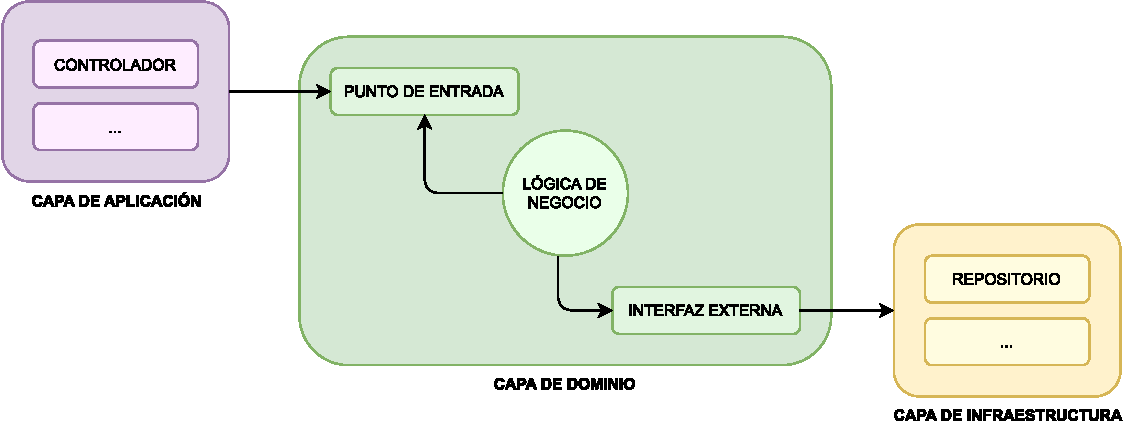
\includegraphics[width=0.9\textwidth]{diagramas/ddd.pdf}
	\caption{Diagrama de capas del patrón de diseño DDD}
	\label{fig:ddd}
\end{figure}

\section{\textit{Frontend}}
\label{sec:herramientas_frontend}

En cuanto al \textit{frontend}, se decidió utilizar NextJS \cite{nextjs} como herramienta para el desarrollo de la interfaz de usuario, dado que ya
se contaba con bastante experiencia previa en su uso. NextJS es un \textit{framework} basado en React \cite{react}, es decir, en la construcción de interfaces dinámicas mediante la composición
de elementos que pueden tener estado. Además, este \textit{framework} implementa varias mejoras sobre React como por ejemplo el \textit{server-side rendering}, algo que ayuda en gran medida
al SEO (del inglés \textit{Search Engine Optimizations}), es decir, a que los motores de búsqueda como Google puedan indexar mejor la página y, por tanto, que esta aparezca en una posición superior en los resultados de búsqueda.
Además, también cuenta con optimizaciones para la carga y el renderizado de imágenes o fuentes entre otras.

\bigskip
Todo ello se desarrolló utilizando TypeScript \cite{typescript}, un lenguaje de programación que añade tipado estático a JavaScript
y que está ganando mucha popularidad con respecto a la mentinibilidad, compresión y escalabilidad que proporciona a los proyectos en los que se usa (Stack Overflow, 2023) \cite{stackoverflow2023}.

\bigskip
En cuanto el estilado de la página, se optó por emplear SASS (del inglés \textit{Syntactically Awesome Style Sheets}) \cite{sass}, un preprocesador de CSS (del inglés \textit{Cascading Style Sheets}) que añade
funcionalidades extra como son el uso de variables, bucles o anidamiento de clases. Además, dado que se estaba desarrollando
una aplicación novedosa, se buscó crear un estilo propio haciendo uso de CSS "nativo", desmarcándose así de librerías que proporcionasen estilos predefinidos como Bootstrap \cite{bootstrap} o componentes ya implementados
como Material UI \cite{materialui} o Chakra UI \cite{chakraui}. Por otra parte, para la creación de gráficos se utilizó la librería ChartJS \cite{chartjs}, una de las más conocidas
y con más soporte en la actualidad. Finalmente, para implementar las animaciones en la interfaz, se hizo uso, en conjunto con las transiciones nativas
de CSS, de Framer Motion \cite{framermotion}, una librería que permite crear animaciones más complejas desde JavaScript/TypeScript. 

\section{Algoritmos de perfilado}
\label{sec:herramientas_algoritmos}

\section{Soporte}
